\documentclass[12pt,a4paper]{report}
\usepackage[utf8]{inputenc}% input encoding
\usepackage[T1]{fontenc}% output encoding
\usepackage{lmodern}% fixes czech letters
\usepackage{textcomp}% right arrow, half
\usepackage[unicode=true,hidelinks,bookmarks]{hyperref}% enable unicode, bookmarks, hide link highlighting
\usepackage{longtable}% multipage tables
\usepackage{graphicx}% images
\usepackage{float}% better floats
\usepackage{enumitem}% list options, numbered items
\usepackage[none]{hyphenat}% prevent hyphenation
\usepackage[normalem]{ulem}% underlines
\usepackage[tmargin=1in,bmargin=1in,lmargin=1in,rmargin=1in]{geometry} % page margins
\usepackage{tabularx}% page-wide table
\newcolumntype{Y}{>{\centering\arraybackslash}X}% content centering in X cell using Y
\newcolumntype{R}{>{\raggedleft\arraybackslash}X}% content right float in X cell using R
\usepackage{helvet}% use Arial/Helvetica clone Nimbus Sans
\usepackage{sectsty}
\allsectionsfont{\sffamily}% use sans-serif font for all sections
\usepackage[parfill]{parskip}
\usepackage{listings}



\lstdefinestyle{code}{
    basicstyle=\ttfamily\footnotesize,
    frame=single
}
\lstset{style=code}
\renewcommand{\contentsname}{Obsah}
\renewcommand{\listfigurename}{Seznam obrázků}
\renewcommand{\figurename}{Obr.}
\renewcommand{\bibname}{Reference}
\renewcommand{\baselinestretch}{1.15}

% custom bibliography
\makeatletter
\renewenvironment{thebibliography}[1]
     {\newpage
     {\Huge \sffamily \bfseries \par\nobreak{\bibname}}% <-- this line was changed from \chapter* to \section*
      \@mkboth{\MakeUppercase\bibname}{\MakeUppercase\bibname}%
      \vskip 40\p@
      \list{\@biblabel{\@arabic\c@enumiv}}%
           {\settowidth\labelwidth{\@biblabel{#1}}%
            \leftmargin\labelwidth
            \advance\leftmargin\labelsep
            \@openbib@code
            \usecounter{enumiv}%
            \let\p@enumiv\@empty
            \renewcommand\theenumiv{\@arabic\c@enumiv}}%
      \sloppy
      \clubpenalty4000
      \@clubpenalty \clubpenalty
      \widowpenalty4000%
      \sfcode`\.\@m}
     {\def\@noitemerr
       {\@latex@warning{Empty `thebibliography' environment}}%
      \endlist}
\makeatother

% custom chapter head
\makeatletter
\renewcommand{\@makechapterhead}[1]{%
\vspace*{0 pt}% 50
{\setlength{\parindent}{0pt} \raggedright \normalfont
\sffamily\bfseries\Huge\thechapter\hspace{1cm}#1
\par\nobreak\vspace{10 pt}}}
\makeatother

\newcommand\T{\rule{0pt}{4ex}}% add space above table row, use before text

% \setlength\parindent{0pt}% remove indentation
\setcounter{secnumdepth}{3}
\setlistdepth{9}%maximal nesting depth

% \tightlist command
\providecommand{\tightlist}{%
\setlength{\itemsep}{0pt}\setlength{\parskip}{0pt}}

\title{Desktopová hra v Unity - Snake Splix}
\author{Vojtěch Svoboda}
\date{}

\begin{document}

\pagenumbering{Roman}

\begin{titlepage}
{\sffamily\bfseries
    \begin{center}
        {\large STŘEDNÍ PRŮMYSLOVÁ ŠKOLA BRNO, PURKYŇOVA,\\\vspace{2mm}
        PŘÍSPĚVKOVÁ ORGANIZACE}\\
        \noindent\rule{\linewidth}{0.4pt}\\
        \vspace{3cm}
        
\includegraphics[width=3.5cm]{images/spseit.png}\\
        \vspace{3cm}
        {\fontsize{24}{28}\selectfont Desktopová hra v Unity - Snake Splix}\\
        \vspace{2cm}
        {\fontsize{16}{20}\selectfont VOJTĚCH SVOBODA}\\
        \vspace{1cm}
        {\fontsize{16}{20}\selectfont V4C}\\
        \vspace{3cm}
        {\fontsize{16}{20}\selectfont PROFILOVÁ ČÁST MATURITNÍ ZKOUŠKY\\\vspace{2mm}
        MATURITNÍ PRÁCE}\\
        \vfill
        {\fontsize{16}{20}\selectfont BRNO 2019}\\
    \end{center}
}
\end{titlepage}

\newpage
\setcounter{page}{2}

\thispagestyle{empty}
\begin{figure}[H]
    \vspace*{-2cm}
    \makebox[\linewidth]{
        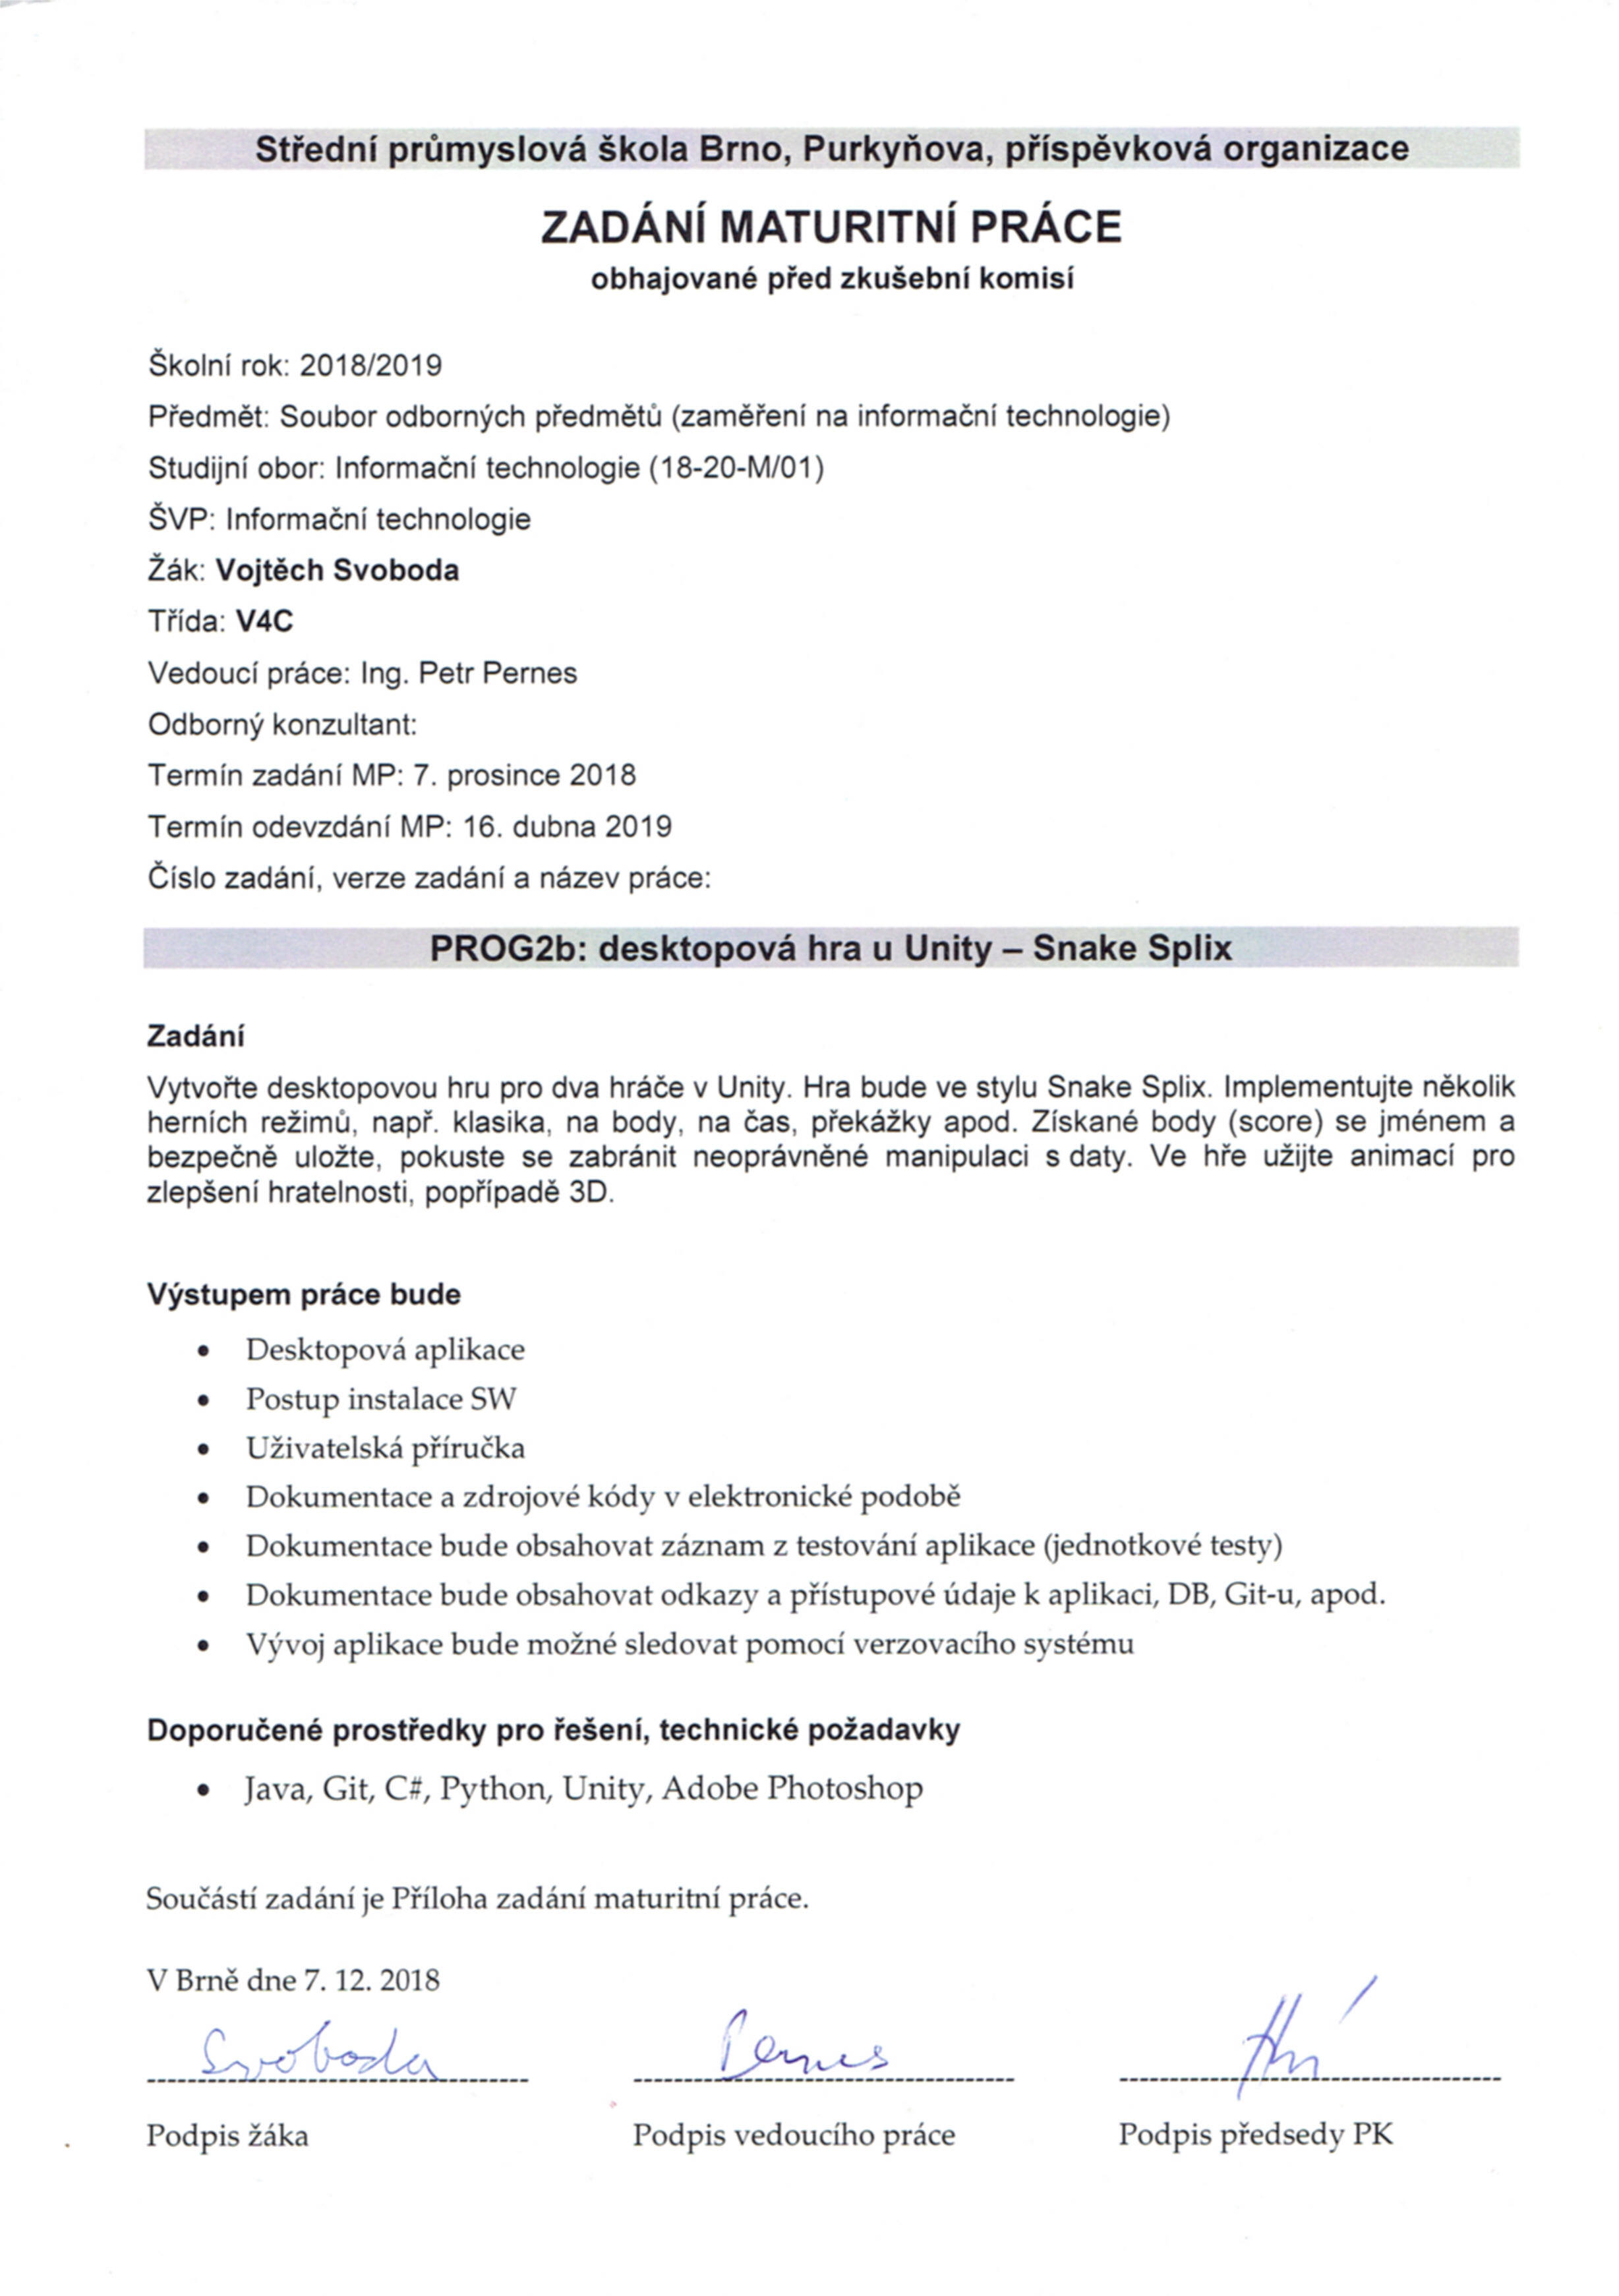
\includegraphics[width=1.2\linewidth]{images/zadani-maturitni-prace.jpg}}
\end{figure}

\newpage

\section*{Prohlášení}
\addcontentsline{toc}{section}{Prohlášení}

\noindent Prohlašuji, že jsem maturitní práci na téma
Desktopová hra v Unity - Snake Splix vypracoval samostatně
a~použil jen zdroje uvedené v~seznamu literatury.\\
Prohlašuji, že:
\begin{itemize}
    \item Prohlašuji, že beru na vědomí, že zpráva o~řešení maturitní práce
    a~základní dokumentace k~aplikaci bude uložena v~elektronické podobě na
    intranetu Střední průmyslové školy Brno, Purkyňova, příspěvkové organizace.
    \item Prohlašuji, že beru na vědomí, že bude má maturitní práce včetně
    zdrojových kódů uložena v~knihovně SPŠ Brno, Purkyňova, p. o., dostupná
    k~prezenčnímu nahlédnutí. Škola zajistí, že nebude pro nikoho možné
    pořizovat kopie jakékoliv části práce.
    \item Prohlašuji, že beru na vědomí, že SPŠ Brno, Purkyňova, p. o., má právo
    celou moji práci použít k~výukovým účelům a~po mém souhlasu nevýdělečně moji
    práci užít ke své vnitřní potřebě.
    \item Prohlašuji, že beru na vědomí, že pokud je součástí mojí práce
    jakýkoliv softwarový produkt, považují se za součást práce i~zdrojové kódy,
    které jsou předmětem\\maturitní práce, případně soubory, ze kterých se práce
    skládá. Součástí práce není cizí ani vlastní software, který je pouze
    využíván za přesně definovaných podmínek, a~není podstatou maturitní práce.
\end{itemize}

\newpage

\section*{Anotace}
\addcontentsline{toc}{section}{Anotace}

\noindent
Tato maturitní práce se zabývá vytvořením počítačové hry pro 2 místní hráče.
Hráči se snaží zabírat území a případně soupeřit s protihráčem v zabírání území.
Hráči mají životy, které ztrácí při naražení do překážky nebo při kolizi s jiným hráčem.
Hra obsahuje i režim pro jednoho hráče.
Ve výsledné práci jsou zvukové efekty, které vylepšují celkový prožitek ze hry. 
Hra je naprogramována v C\# a jako herní engine bylo použito Unity.


\subsection*{Klíčová slova}

\emph{unity, hráč, herní engine, C\#, zabraná oblast}

%%\section*{Annotation}
%%\addcontentsline{toc}{section}{Annotation}

%%\noindent
%%A goal of this project was to create a game for 2 local players.

%%\subsection*{Keywords}

%%\emph{keywords}

\newpage

\pagenumbering{arabic}

\setcounter{page}{5}


\begingroup
\makeatletter
% Redefine the \chapter* header macro to remove vertical space
\def\@makeschapterhead#1{%
  %\vspace*{50\p@}% Remove the vertical space
  {\parindent \z@ \raggedright
    \normalfont
    \interlinepenalty\@M
    \Huge \sffamily \bfseries  #1\par\nobreak
    \vskip 40\p@
  }}
\makeatother

\tableofcontents
\endgroup
%%\tableofcontents
%%\addcontentsline{toc}{section}{Obsah}

\begingroup
\makeatletter
% Redefine the \chapter* header macro to remove vertical space
\def\@makeschapterhead#1{%
  %\vspace*{50\p@}% Remove the vertical space
  {\parindent \z@ \raggedright
    \normalfont
    \interlinepenalty\@M
    \Huge \sffamily \bfseries  #1\par\nobreak
    \vskip 40\p@
  }}
\makeatother

\listoffigures
\endgroup

%%\listoffigures
%%\addcontentsline{toc}{section}{Seznam obrázků}

\chapter*{Seznam použitých zkratek}
\addcontentsline{toc}{section}{Seznam použitých zkratek}

\begin{tabularx}{\textwidth}{l@{\hskip 2cm}X}
    \textbf{C\#} & C Sharp; programovací jazyk \\
    \T \textbf{GameObject} & Objekt v herním prostředí, má atributy a svoji polohu v herním prostředí \\
    \T \textbf{AudioMixer} & V audio mixeru se přidávají skupiny zvuků, kterým lze měnit hlasitost \\
    \T \textbf{UI} & User Interface; uživatelské rozhraní \\
    \T \textbf{Alpha} & Parametr průhlednosti barvy \\
    \T \textbf{Vector3} & Odkazuje na přesné místo v herním prostředí; vypočítá se z x,y,z souřadnic \\
    \T \textbf{Herní engine} & Sada komponent, které zjednodušují práci při výrobě počítačových her \\
    \T \textbf{LaTeX} & Lamport TeX; program pro počítačovou sazbu; za pomoci něj jdou psát dokumenty \\
    \T \textbf{GitHub} & Verzovací online systém \\
    \T \textbf{Tick} & Jeden snímek v herním prostředí \\
    \T \textbf{Ocas} & Cesta, kterou za sebou zanechává hráč; Pokud přes ni přejede oponent ztratí hráč život \\
\end{tabularx}

\chapter{Teoretický úvod}
Celá maturitní práce je dostupná na: \href{https://github.com/vojtas131/Snake-Splix-Public}{github.com/vojtas131/Snake-Splix-Public} a uživatelská aplikace je pod záložkou release.
\section{Výběr tématu}
Téma jsem si vybral, protože mě baví hry a baví mě je programovat.
S herním enginem Unity už jsem věděl základy, takže jsem nemusel řešit orientaci v prostředí a učit se základy C\#.

\section{Cíl práce}
Cílem práce je vytvořit hru, ve které se mohou zabavit 2 hráči a soutěžit spolu. Hra by měla být zábavná a správně vybalancovaná.
Vedlejším cílem bylo vytvořit mód pro 1 hráče, kde hráč zápasí s časem a vyhýbá se překážkám.
\chapter{Rozbor řešení}
\section{Rozbor problémů}
\subsection{Vyplnění pole}
Jako základ funkčnosti bylo navrhnout algoritmus, který by vyplňoval pole, které hráč zabere.
Problém je, že hráč může obsadit pole různých tvarů a proto bylo potřeba, aby algoritmus pokryl všechny možnosti.
\subsection{Vytváření herních objektů}
Bylo potřeba zachovat ve všem sounáležitost.
Tedy mapa, hráčova oblast a hráči museli spolupracovat spolu a být na sobě nezávislé.
\subsection{Balance a zábava hry}
Tento problém byl spíš po stránce game designu než kódu.
Bylo potřeba vyřešit, aby zbývající životy měli určitý vliv na skóre.
\subsection{Zabíjení mezi hráči}
Problém se skládal ze 2 částí. Kdy má hráč umřít a kdo umře pokud se hráči srazí.
\section{Použitá technologie}
\subsection{Unity}
Jako herní engine jsem použil Unity.
I když jsem měl na výběr i z jiných herních enginů (jako například Unreal engine nebo Cryengine),
Unity mi přišlo nejlepší, protože jsem v něm už pracoval.
Programovací jazyk pro scripty je v C\#.
Ačkoliv Unity podporuje i JavaScript, je už na ústupu a nedoporučuje se používat.
\newpage
\subsection{Bosca Ceoil}
Potřeboval jsem program, ve kterém mohu jednoduše vytvořit hudbu. Bosca Ceoil splnil všechny tyto podmínky a je navíc zdarma.
\newline
\begin{figure}[H]\centering
    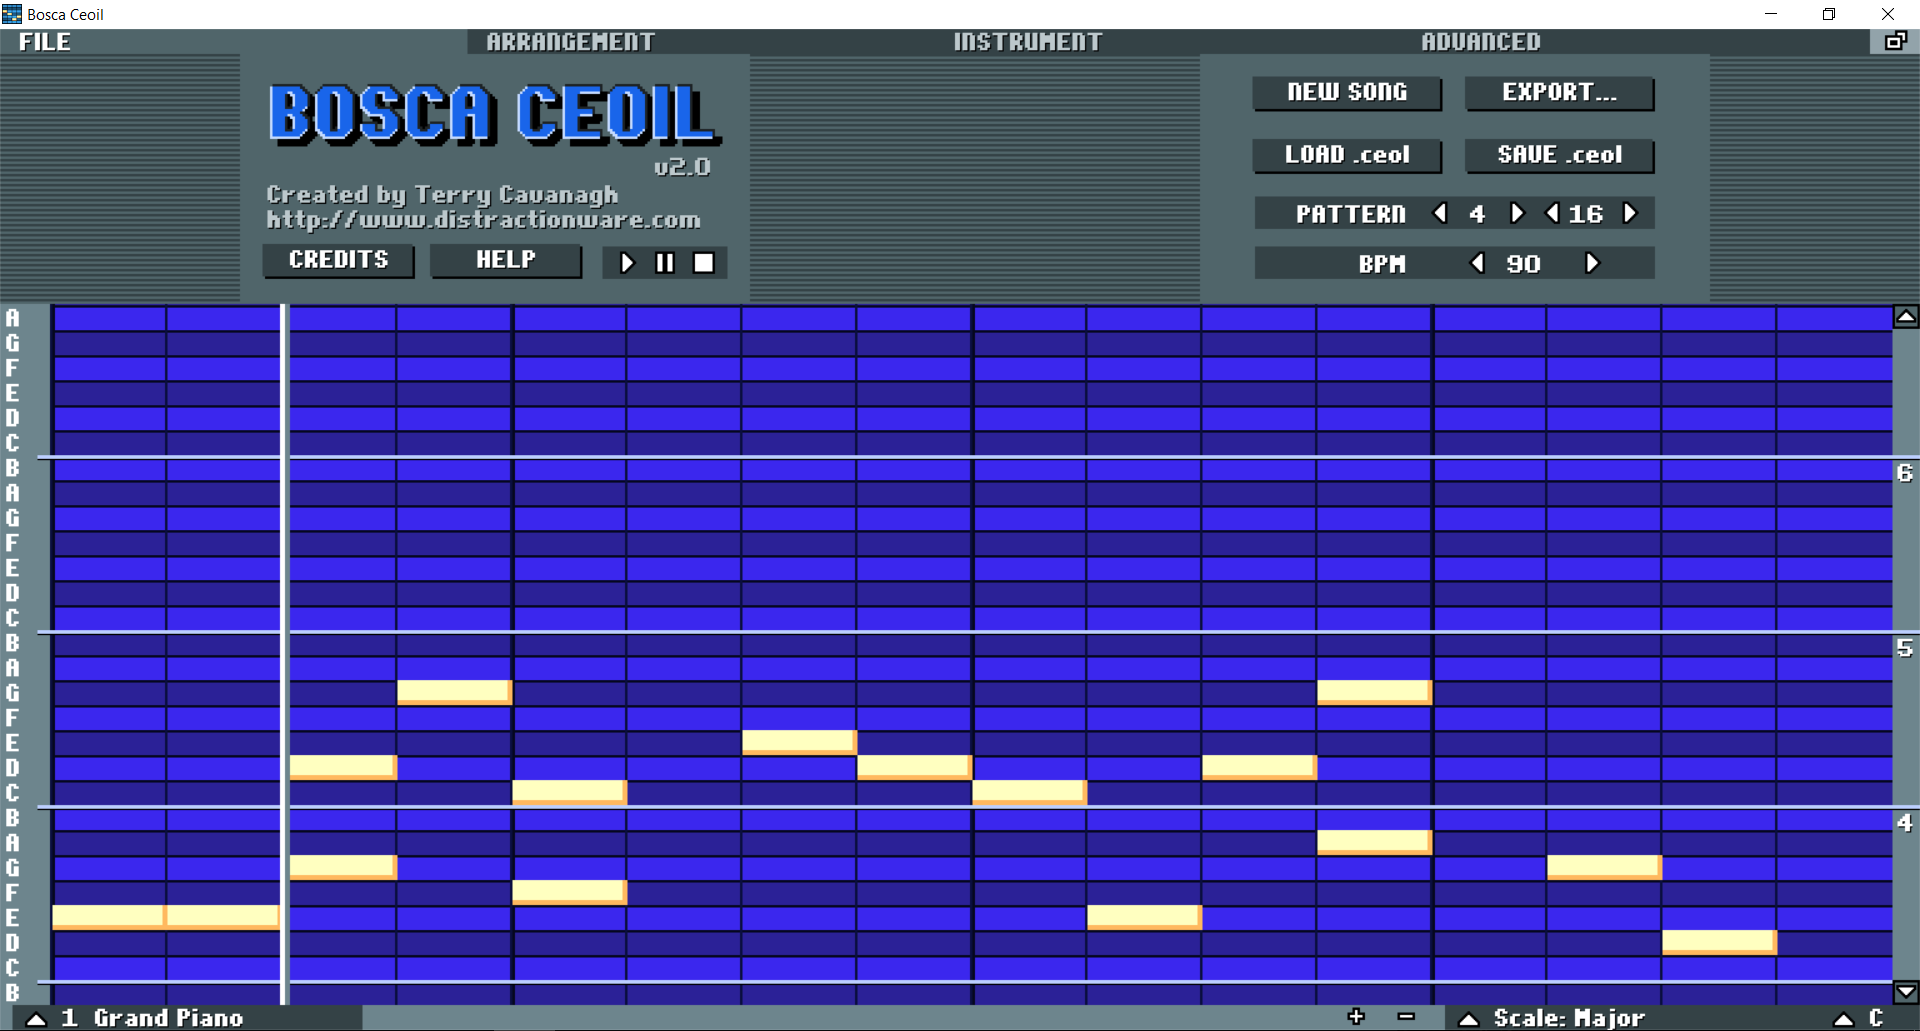
\includegraphics[width=\textwidth]{images/bosca_ceoil.png}
    \caption{Prostředí programu Bosca Ceoil}
\end{figure}
\chapter{Assety}
\section{Skripty}
\subsection{AudioManager.cs}
Skript slouží k ovládání audia skrz scény. Je dán na GameObject, který se přenáší skrz scény.
Pracuje s atributy Sound.cs.
\subsection{GameManager.cs + GameManager2P.cs}
Slouží k funkčnosti hry, je rozdělen na mód pro jednoho hráče a na mód pro dva hráče.
Tento skript je pro jeho rozsáhlost vysvětlen v kapitole
\hyperref[sec:gamemanager]{4.GameManager} na stránce \pageref*{sec:gamemanager}.
\subsection{MainMenu.cs}
Jsou v něm metody pro funkčnost a chod Hlavního menu.
Skript dělím na regiony, ve kterých definuji funkce, pro různé části menu. \\
\textbf{Customization} \\
Neboli přizpůsobení herních prvků.
\begin{lstlisting}
public void ApplyChanges(){
    warning.SetActive(false);
    if(Int32.Parse(inputObstacles.text)
        >=(((Int32.Parse(inputHeight.text)-3)
        *(Int32.Parse(inputWidth.text)-3))-8)){
        warning.SetActive(true);
        return;
    }
    StartCoroutine(ApplyChangesCoroutine());
}
\end{lstlisting}
Tato metoda se volá při stisku tlačítka Apply changes.
Testuji aby počet překážek nebyl větší než maximální počet překážek na mapu.
\\
Vzorec je ((výška celé mapy)-3)*((šířka celé mapy)-3) - 8 (což je počet startovních polí pro hráče).
Poté se volá ApplyChangesCoroutine(), která obsahuje metody, abych vytvořil zpoždění.
\newpage
\begin{lstlisting}
public IEnumerator ApplyChangesCoroutine(){
    saved.GetComponent<Text>().color = new Color(0,0,0,255);
    saved.SetActive(true);
    ...
    saved.GetComponent<Text>().CrossFadeAlpha(0,1.5f,false);
    yield return new WaitForSeconds(1.5f);
    saved.SetActive(false);
    yield return null;
}   
\end{lstlisting}
Pro vytvoření textu, který postupně mizí, jsem použil alpha parametr v barvě textu.
Použil jsem metodu CrossFadeAlpha, která postupně mění alphu v barvě textu.
Nastavil jsem dobu trvání na 1.5~s.
Poté celá funkce čeká stejnou dobu a pak nastaví text na neviditelný.
\subsection{Node.cs}
Odkazuje na jedno pole na mapě. Je v něm poloha x, y, jeho worldPosition (místo v herním prostředí), komu políčko patří a jestli na něm právě je nebo není ocas hráče.
\begin{lstlisting}[]{}
public class Node{
    public int x;
    public int y;
    public Vector3 worldPosition;
    public int land;
    public int tail;
}
\end{lstlisting}
Čerpá z něho:
\begin{itemize}
    \item   HelpNode.cs - Pomocná třída při barvení oblasti, kterou hráč zabral.
    \item   LandNode.cs - Je v něm herní objekt, pole, a komu patří pole.
    \item   TailNode.cs - Je v něm herní objekt a pole.
\end{itemize}
\subsection{Sound.cs}
Třída která určuje parametry zvuků ve hře.
Má zdrojový zvuk, hlasitost, výšku, opakování a ke kterému AudioMixeru patří.
\section{Models}
\subsection{Model hráče, mapa}
Protože modely hráče a mapy dělám jenom z barvy, nebylo potřeba vytvořit modely pro tyto objekty v externím programu.
\subsection{Slider}
Pro posuvník hudby jsem potřeboval model. Vyrobil jsem tento jednoduchý obrázek 32x32 pixelů.
Tento model jsem vytvořil v online programu Piskel.
\begin{figure}[H]\centering
    
\includegraphics[]{images/SliderCube.png}
    \caption{Slider Cube}
\end{figure}
\section{Audio}
Jako hudbu jsem se inspiroval 8-bitovou. \\
Vytvořil jsem zvuky pro:
\begin{itemize}
    \item Smrt - Death.wav
    \item Výhru - Victory2.wav
    \item Vybarvení pole - Fill.wav
    \item Hudba do pozadí - MainMenuMusicTheme4.wav
\end{itemize}
\section{Fonts}
Jako font jsem použil font s nádechem 8-bitových her. Použil jsem font PressStart2P.ttf.
\begin{figure}[H]
    \centering
    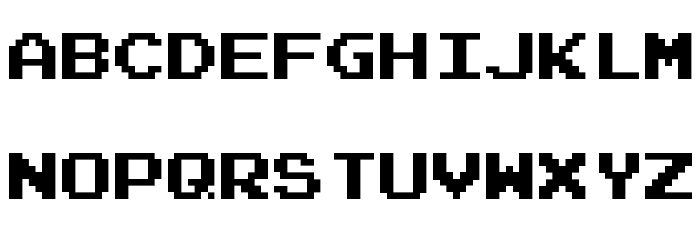
\includegraphics[width=.8\textwidth]{images/Press-Start-2PA.png}
    \caption{PressStart2P.ttf}
\end{figure}

\newpage
\section{Scenes}
\subsection{MainMenu.unity}
Jsou na ní tlačítka na zvolení herního módu, nastavení, o autorovi a na odejití ze hry.

\begin{figure}[H]\centering
    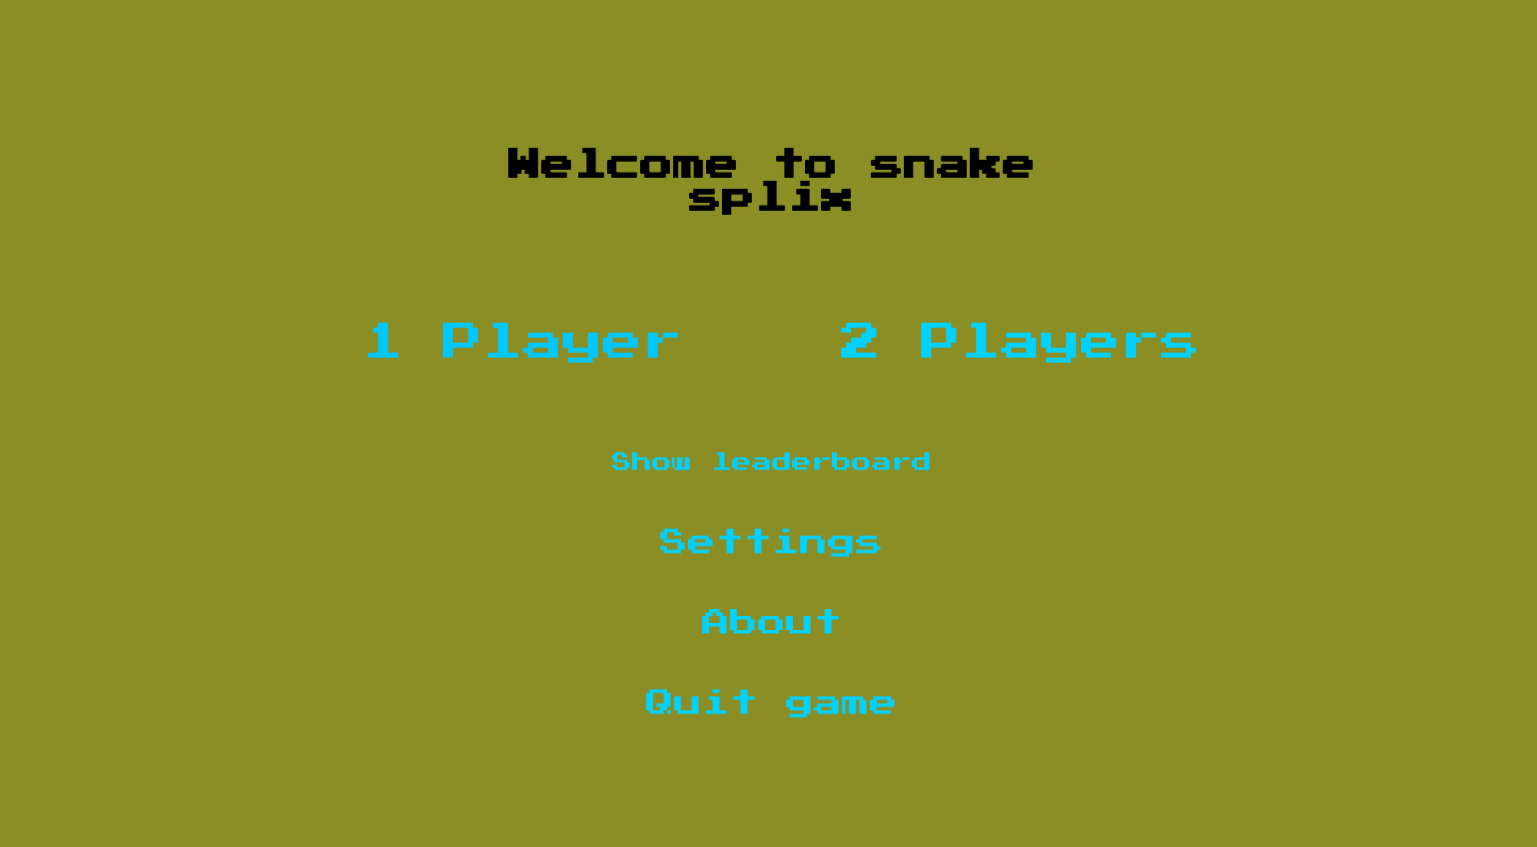
\includegraphics[width=.9\textwidth]{images/main_menu.png}
    \caption{Main menu}
\end{figure}
\subsection{GameP1.unity + GameP2.unity}
Scéna ve které probíhá hra. Má hráče, mapu a UI prvky které ukazují životy, skóre a čas.
\begin{figure}[H]\centering
    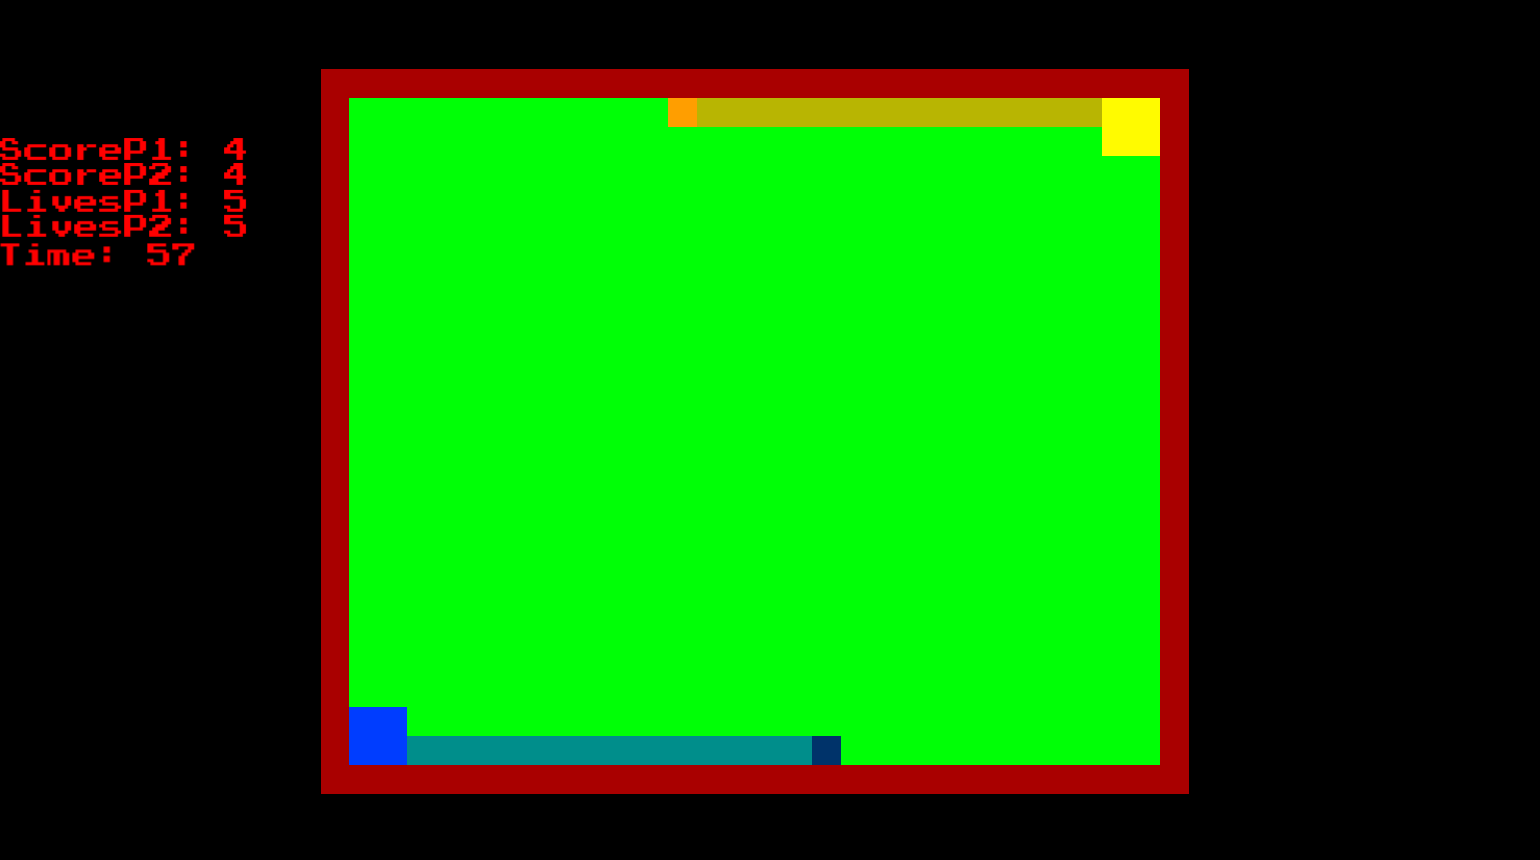
\includegraphics[width=.9\textwidth]{images/game.png}
    \caption{Hra pro 2 hráče}
\end{figure}
\chapter{GameManager.cs}
\label{sec:gamemanager}
\section{Update()}
Update metoda se volá každý tick. 
\begin{lstlisting}[]{}
void Update(){
    if(!gameover){
        if(Input.GetButtonDown("Esc")){ 
            pause ^= true;
            Cursor.visible ^= true;
        }
        if(!pause){
            pauseMenu.SetActive(false);
            GetInput();
            SetPlayerDirection();
            timer += Time.deltaTime;
            time -= Time.deltaTime;
            if (timer > moveRate){
                timer = 0;
                curDirectionP1 = targetDirectionP1;
                curDirectionP2 = targetDirectionP2;
                MovePlayer();
            }
            curTimeText.text = "Time: " + Mathf.Round(time).ToString();
            if(time<=0) ResetPlayer();
        }
        else if(pause){
            pauseMenu.SetActive(true);     
        }
    }
}
\end{lstlisting}
Hra se zastaví při stisku klávesy Esc. "pause" změní svoji hodnotu a kurzor myši je viditelný. \\
Update metoda funguje při každém ticku (snímku). Volá se GetInput() která zjišťuje které klávesy byli stisknuty.
V každém ticku se přenáší hodnota reálného času do proměnné "timer".
Jakmile "timer" získá hodnotu větší než je nastaven v "moveRate", tak zavolá metodu na pohyb hráče a "timer" se vynuluje.
SetPlayerDirection() nastaví směr každého hráče. Získávám dvě "curDirection" pokud se jedná o hru pro dva.
\section{Pohyb hráče}
Nejdříve se zjistí, kterým směrem hráč jede.
Pak se nastaví hodnota x nebo y podle směru.
\begin{lstlisting}
Node targetNodeP1 = GetNode(player1Node.x + P1x, player1Node.y + P1y);
Node targetNodeP2 = GetNode(player2Node.x + P2x, player2Node.y + P2y);
player1.transform.position = targetNodeP1.worldPosition;
player1Node = targetNodeP1;
if (player1PrevNode.land != 1) {
    tailP1.Add(CreateTailNodeP1(player1PrevNode.x, player1PrevNode.y));
    player1PrevNode.tail = 1;
}
\end{lstlisting}
Zjistí se následující pole, na kterém se hráč bude nacházet.
Hráčova pozice se nastaví na následující pole pomocí ".transform.position".
Jestliže hráčovo předchozí pole bylo jeho vlastní, ocas se nevytvoří.
To stejné se provádí i pro druhého hráče.
\begin{lstlisting}
if (targetNodeP1.land == 1 && tailP1.Count > 0) {
    int countTail = tailP1.Count;
    FindObjectOfType<AudioManager>().PlayOneShot("Fill");
    for (int i = 0; i < countTail; i++) {
        TailNode curr = tailP1[0];
        curr.node.tail=0;
        CreateLandNodeP1(curr.node.x, curr.node.y);
        RemoveTail(tailP1);
    }
    FillP1();
    UpdateScore();
}
\end{lstlisting}
Pokud hráč skončí ve svém poli tak se začne vybarvovat jeho pole.
Nejdříve vybarvím ocas a pak vybarvím oblast uvnitř.
\section{Problematika vybarvení hráčova pole}
Při řešení problému jak vybarvit část, kterou hráč zabral, jsem musel vytvořit vhodný algoritmus.
\begin{lstlisting}[]{}
void FillRest(Node node){
    if(node.land==2) return;
    if(node.land==1) return;
    landP1.Add(CreateLandNode(node.x, node.y));
    FillRest(GetNode(node.x,node.y+1));
    FillRest(GetNode(node.x,node.y-1));
    FillRest(GetNode(node.x-1,node.y));
    FillRest(GetNode(node.x+1,node.y));
}  
\end{lstlisting}
Algoritmus pro vybarvení jsem měl hned. 
Stačilo zvolit pole uvnitř oblasti a metoda vytvářela hráčova pole, dokud nenarazila na ocas nebo na hráčovo už zabrané pole.
Při každém projití se metoda zavolá znovu se sousedními poly.
Problém byl ten, že bylo zapotřebí zjistit jedno z polí, které se nachází uvnitř hráčovi oblasti.
Další problém byl ten, že pokud by hráč vytvořil podobnou oblast jako je na \hyperref[fig:dvepole]{Obr. 4.1}, tak by bylo potřeba najít pole v obou oblastech. 
\begin{figure}[H]\centering
    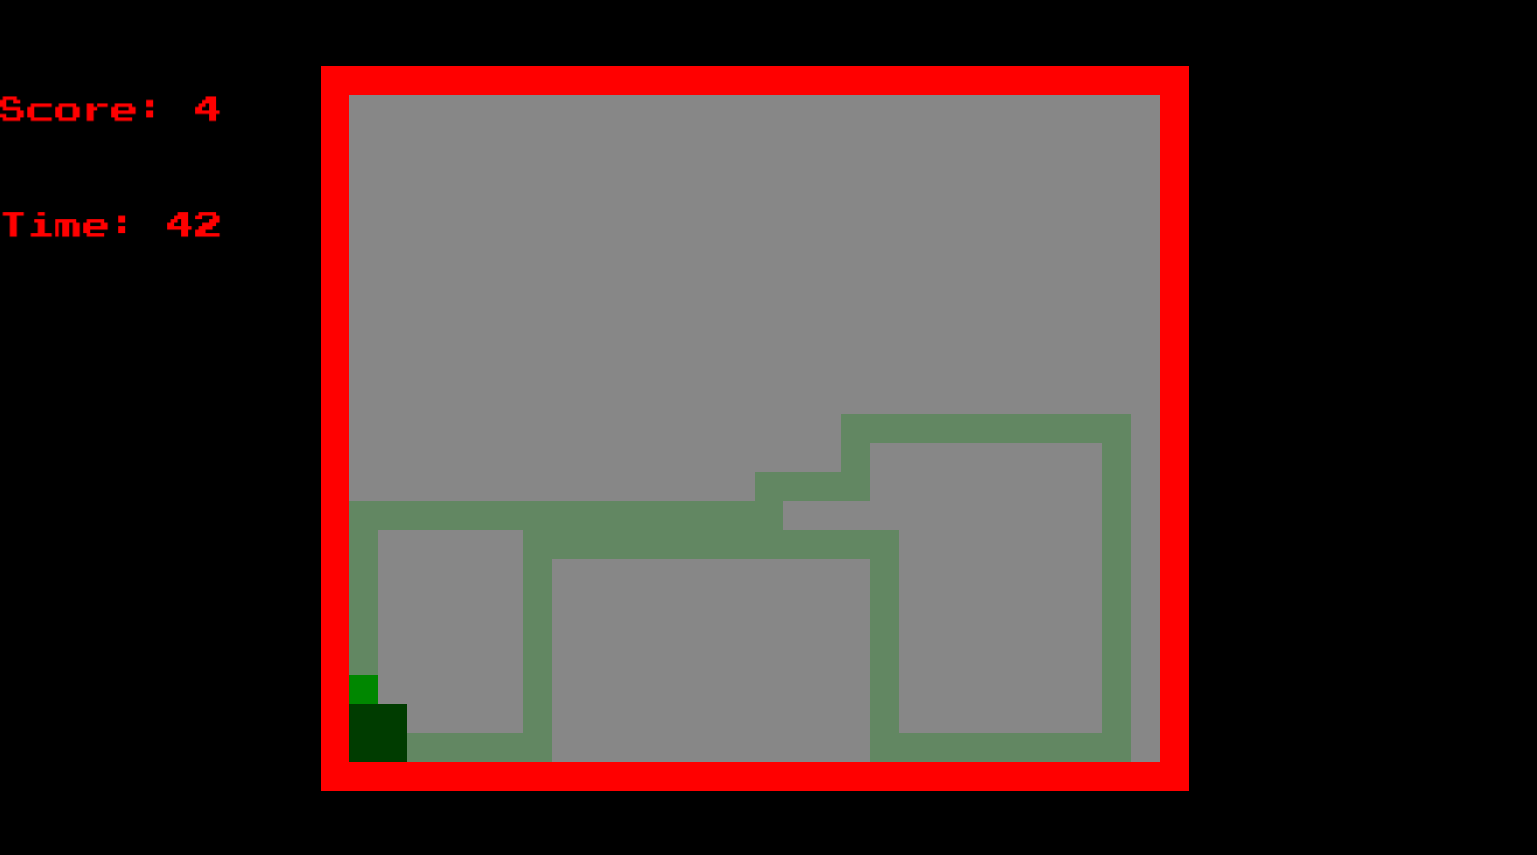
\includegraphics[width=\textwidth]{images/dvepole.png}
    \caption{Možnost hráče jak vybarvit pole}
    \label{fig:dvepole}
\end{figure}
V první verzi hry tedy hráč musel specificky ukončit oblast, aby se správně vybarvila.
\\\\
Použil jsem tedy jiný způsob na vybarvení pole a to inverzním způsobem.
Vytvořil jsem novou mapu, která se tentokrát skládala z HelpNode.
HelpNode třída má Node a pomocný parametr own (ownership = vlastnictví).
\begin{lstlisting}[]{}
void HelpFill(HelpNode node){
    if (node == null) return;
    if (node.node.land == 1) {
        node.own = 1;
        return;
    }
    if (node.own == -1) return;
    node.own = -1;
    HelpFill(GetHelpNode(node.node.x, node.node.y + 1));
    HelpFill(GetHelpNode(node.node.x, node.node.y - 1));
    HelpFill(GetHelpNode(node.node.x - 1, node.node.y));
    HelpFill(GetHelpNode(node.node.x + 1, node.node.y));
}
\end{lstlisting}
Procházel jsem novou mapu stejným způsobem, jako když jsem vytvářel vytvářel hráčovo pole,
ale tentokrát místo vytvoření pole, jsem měnil parametr own na -1 (mimo), nebo na 1 pokud narazil na hráčovo území.
\begin{lstlisting}[]{}
void FillRest() {
    for (int i = 0; i < maxWidth; i++) {
        for (int j = 0; j < maxHeight; j++) {
            if ((GetHelpNode(i, j)).own == 0) {
                CreateLandNode(i, j);
            }
        }
    }
}
\end{lstlisting}
Pak stačí projít mapou a na všech pozicích, kde se parametr nezměnil, vytvořit hráčovo pole.
Metoda CreateLandNode() je ještě opatřena testem, jestli není hráčovo pole již na tomto poli vytvořeno (aby nevznikli duplikáty).
\section{Leaderboard}
Leaderboard je žebříček nejlepších hráčů. Hráč musí získat větší skóre než nejhorší hráč, aby se dostal na žebříček.
\begin{lstlisting}
    string input = inputName.text;
    if(input.Contains(",") || input.Contains(";"))     return;
    string scores = PlayerPrefs.GetString("highscores",";");
    string[] scoresAndNames = new string[2];
    scoresAndNames = scores.Split(';');
    string[] scoresList = new string[11];
    scoresList = scoresAndNames[0].Split(',');
    string[] namesList = new string[11];
    namesList = scoresAndNames[1].Split(',');
\end{lstlisting}
Highscores jsou uloženy jako řetězec v registrech. Pokud neexistuje vytvoří se s hodnotou ";".
Načítá se pod klíčem "highscores". 
V první části jsou uloženy skóre, v druhé jména (odděleno ";" a hodnoty v řetězci ",").
Pokud by jméno obsahovalo jeden z těchto znaků, tak se vrátí a nenechá hráče vytvořit takové jméno.
\newpage
\begin{lstlisting}  
    for(int i=0;i<scoresList.Length;i++){
        bool emptyField = Int32.TryParse(scoresList[i],out int x);
        if(!emptyField){
            namesList[i]=input;                
            scoresList[i]=score.ToString();
            break;
        }
        if(score>=x){
            for(int n=scoresList.Length-1;n>i;n--){
                scoresList[n]=scoresList[n-1];
                namesList[n]=namesList[n-1];    
            }
            scoresList[i]=score.ToString();
            namesList[i]=input;
            break;
        }
    }
\end{lstlisting}
Převádím skóre ze stringu na int. Pokud nejde převést (pole obsahuje "") metoda TryParse() vyhodí false.
Nejvyšší skóre je uloženo na začátku. Jakmile je hráčovo aktuální skóre větší než uložená hodnota, tak se všechny hodnoty posunou o 1 dolů.
\begin{lstlisting}
    string listOut = "";
    int length;
    if(scoresList.Length>=10)    length = 10;
    else length = scoresList.Length;
    for(int i=0;i<length;i++){ 
        listOut += scoresList[i]+",";
    }
    listOut += ";";        
    for(int i=0;i<length;i++){
        listOut += namesList[i]+",";
    }
    PlayerPrefs.SetString("highscores",listOut);
\end{lstlisting}
Následně převedu všechny hodnoty zpět do jednoho stringu ve stejném formátu jako jsem string načítal.
Uložím do registru pod klíčem "highscores".
\newpage
\section{Kdy hráč umře}
Aby byla hra více zábavná ve dvou hráčích, přidal jsem možnost zabíjení se mezi sebou.
S tím však přišly problémy typu, kdo má umřít pokud se hráči srazí přímo.
\begin{lstlisting}
if(player1Node == player2Node){
    if(player2Node.land==3){
        killP1=true;
    }
    else if(player1Node.land==1){
        killP2=true;
    }
    else{
        killP1=true;
        killP2=true;
    }
}
\end{lstlisting}
Pokud se hráči budou nacházet oba na stejném poli, tak by měli oba umřít.
Dal jsem ale tomu hráči, který se bude nacházet uvnitř svého pole, výhodu.
Díky tomu přežije ten hráč, který je uvnitř své vybarvené oblasti, pokud se oba hráči srazí.
Pokud se oba hráči srazí mimo své pole, tak umřou oba.
\begin{lstlisting}
if(player2Node.tail == 1)   killP1=true;
if(player1Node.tail == 2)   killP2=true;

if(player1Node.tail == 1 || player1Node.land == -1 
    || player1Node.land == 2 || player1Node.land == 4){
    scoreP1-=5;
    ResetPlayer(false);
}

if(player2Node.tail == 2 || player2Node.land == -1 
    || player2Node.land == 2 || player2Node.land == 4){
    scoreP2-=5;
    ResetPlayer(true);
}   
\end{lstlisting}
V první části kódu zjišťuji, jestli se některý z hráčů nenachází na ocasu druhého hráče.
Pokud tomu tak je, tak druhý hráč zemře.
V druhé části kódu zjišťuji, jestli se hráč nezabil sám.
K tomu může dojít, pokud hráč trefí překážku, nebo když trefí svůj vlastní ocas.
Ještě ke všemu ztratí 5 bodů ze skóre.
Pokud umřel druhý hráč díky prvnímu hráči, přičte se mu ke skóre 5 bodů.
\newpage
\section{Ztracení životů}
Pro 2 hráče jsou 2 metody, jedna při úmrtí a druhá při skončení hry.
V případě jednoho hráče stačila jedna metoda na prohru, protože hráč má jen jeden život.
\begin{lstlisting}
private void ResetPlayer(bool player){
    if(!player){
        livesP1--;
        int countTailP1 = tailP1.Count;
        for(int i=0;i<countTailP1;i++){
            tailP1[0].node.tail=0;
            RemoveTail(tailP1);
        }
        int listInt = rnd.Next(0,landP1.Count-1);
        player1Node = landP1[listInt].node;
        player1.transform.position = player1Node.worldPosition;
        Node player1NodeRight = GetNode(player1Node.x+1,player1Node.y);
        if(player1NodeRight.land==-1 
            || player1NodeRight.land==2 
            || player1NodeRight.land==4){
                targetDirectionP1 = Direction.left;
            }
        else    targetDirectionP1=Direction.right;
    }
\end{lstlisting}
Proměnná "player" říká, který z hráčů umřel (false = Hráč 1;true = Hráč 2).
Hráči se odečtou životy a poté se na každé pole, kde měl hráč ocas, zavolá metoda RemoveTail(),
kde se odebere část ocasu a změní v poli hodnotu "tail" na 0.
Následně se vybere jedno náhodné pole, které hráč vlastní a oživí ho zde.
Jestli by bylo pole hned vedle překážky, bude směr hráčova pohybu doleva.
\begin{lstlisting}
void GameOver(){
    FindObjectOfType<AudioManager>().Play("PlayerWin");
    finalScoreP1+=livesP1*10;
    finalScoreP2+=livesP2*10;
    gemeoverMenu.SetActive(true);
    if(finalScoreP1==finalScoreP2){
        gameoverMessage.text = "TIE";
    }
    else if(finalScoreP1<finalScoreP2){
        gameoverMessage.text ="P2 WIN";
        matchesWonP2++;
    }
    else if(finalScoreP1>finalScoreP2){
        gameoverMessage.text ="P1 WIN";   
        matchesWonP1++;
    }
    matchesScoreP1.text=matchesWonP1.ToString();
    matchesScoreP2.text=matchesWonP2.ToString();
\end{lstlisting}
Metoda GameOver() se volá pokud jednomu z hráčů dojdou životy, nebo vyprší čas.
Přehraje se zvuk vítězství, pak se převedou zbývající hráčovi životy na skóre.
Následně se porovnají skóre a vítězovi se přidá vyhraný zápas.
Pokud hráči hrají víckrát, pak se číslo vyhraných zápasů zvětšuje.
V případě remízy se nepřičte vyhraný zápas ani jednomu.

\chapter{Závěr}
V maturitní práci se mi bohužel nepovedlo začlenit animace, protože jsem nevěděl, jak je zakomponovat do takto graficky jednoduché hry.
Zabezpečení highscore je pouze v registru a tak se k tomu někteří uživatelé můžou dostat.
Ostatní požadavky zadání jsem splnil. 
\\\\
Díky maturitní práci jsem si vylepšil znalosti s herním enginem unity a jazyka C\#.
Pokud bych maturitní práci dělal teď, napsal bych kód určitě jinak (například bych raději udělal jeden skript pro mód 1 hráče i pro 2).
Bohužel na kompletní přepsání nemám dostatek času.
\\\\
Pokud bych se k této maturitní práci v budoucnu vrátil, určitě bych dodělal lepší zabezpečení dat a přidal různé drobnosti.
Mezi drobnosti bych uvedl například herní měnu, různé hráčovi barvy, levely a s nimi zvětšující se obtížnost, nepřátelé.
I přes tyto drobnosti dopadla maturitní práce podle mých představ a jsem s výsledkem spokojený. 
\\\\
Výslednou dokumentaci jsem vytvořil v LaTeXu a kód je dostupný na githubu ve složce Documentation.

\begin{thebibliography}{10}
    \bibitem{Polozka1} Press Start 2P Font | dafont.com. DaFont - Download fonts [online]. Dostupné z: \url{https://www.dafont.com/press-start-2p.font}
    \bibitem{Polozka2} Unity - Manual: Unity User Manual (2018.3). [online]. Copyright © 2019 Unity Technologies. Publication [cit. 06.04.2019]. Dostupné z: \url{https://docs.unity3d.com/Manual/index.html}
    \bibitem{Polozka3} Průvodce jazykem C\# | Microsoft Docs. [online]. Dostupné z: \url{https://docs.microsoft.com/cs-cz/dotnet/csharp/}
    \bibitem{Polozka4} Bosca ceoil. Home [online]. Dostupné z: \url{https://boscaceoil.net/}
    \bibitem{Polozka5} Piskel - Free online sprite editor. Piskel - Free online sprite editor [online]. Dostupné z: \url{https://www.piskelapp.com/}
    \bibitem{Polozka6} LaTeX - A document preparation system. LaTeX - A document preparation system [online]. Dostupné z: \url{https://www.latex-project.org/}
\end{thebibliography}

\chapter{Příloha - Uživatelská příručka}

\vspace*{\fill}
{\sffamily\bfseries
    \begin{center}
        {\fontsize{24}{28}\selectfont UŽIVATELSKÁ PŘÍRUČKA}
    \end{center}
}
\vspace*{\fill}
\chapter{Úvod}
Snake Splix je 2D hra pro jednoho nebo dva hráče.
Jako čtvereček jedné určité barvy se budete snažit zabírat území, vyhýbat se překážkám a případně vyhrát nad protihráčem.
Pokud se vám bude dařit, můžete své skóre uložit do seznamu nejlepších hráčů.
Jakmile se začnete nudit, můžete změnit velikost mapy, rychlost hry a jiné herní prvky.
\par
{\let\clearpage\relax 
\chapter{Uživatelské rozhraní}}
Při zapnutí hry vás přivítá toto menu.
\begin{figure}[H]\centering
    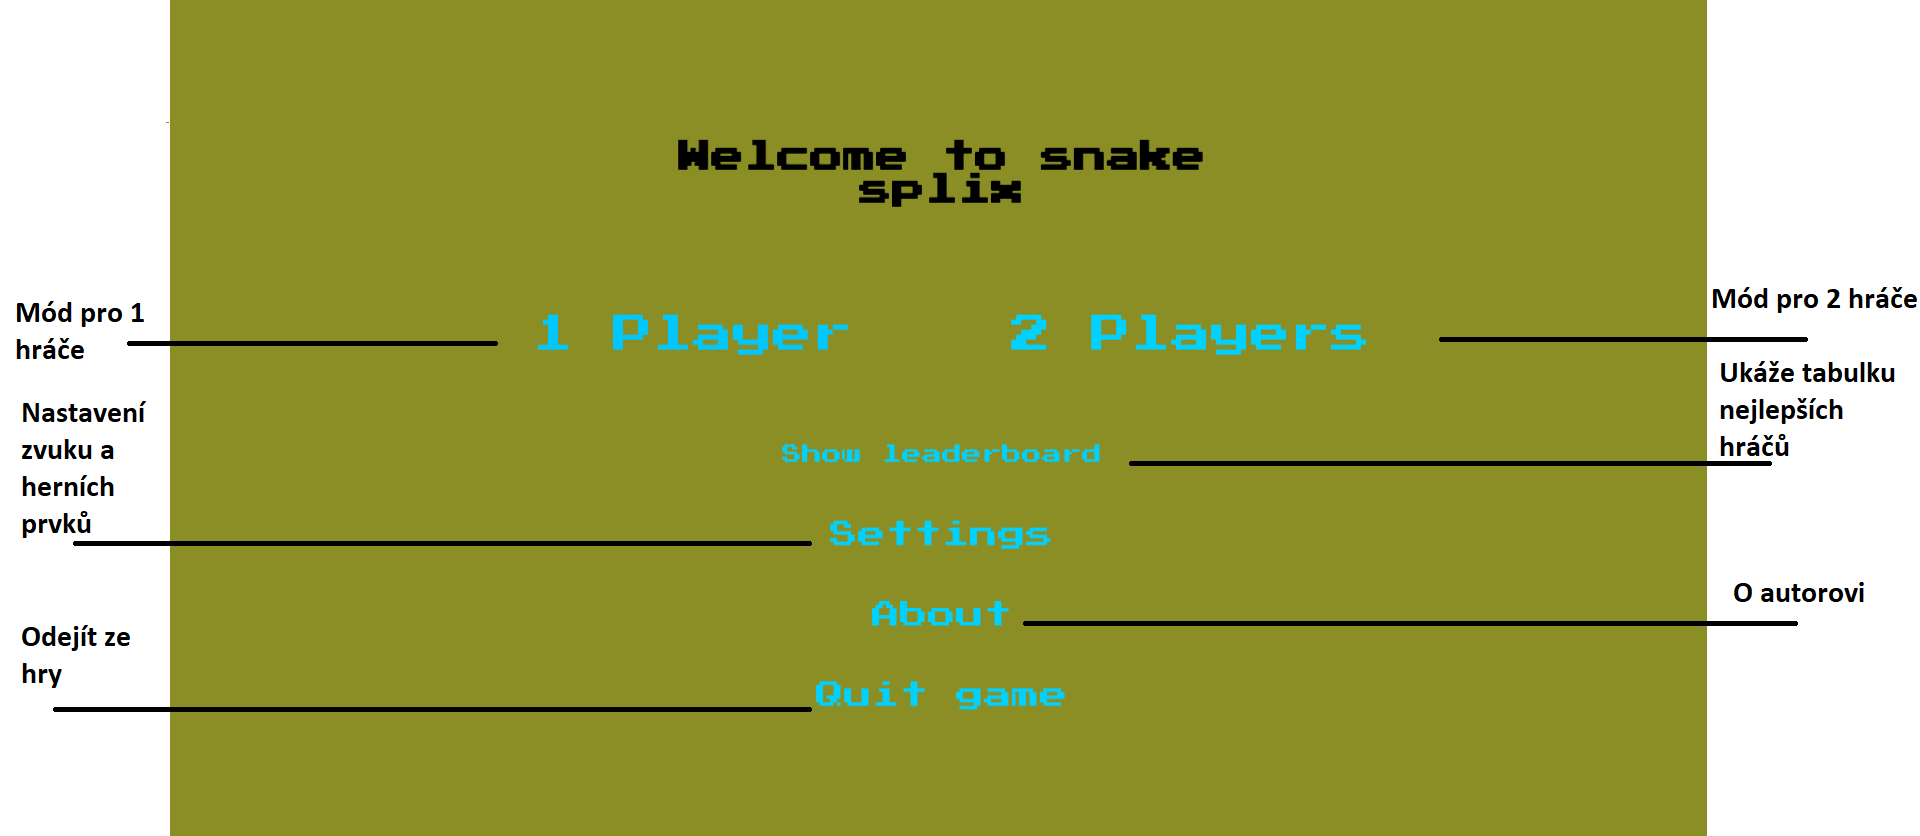
\includegraphics[width=\textwidth]{images/main_menu_desc.png}
    \caption{Hlavní menu}
\end{figure}
Pokud chcete hrát sami stiskněte 1 Player (1 hráč) a pokud chcete hrát ve 2 stiskněte 2 Players (2 hráči). \\
Pokud se chcete podívat na seznam nejlepších hráčů, můžete tak udělat kliknutím na tlačítko Show leaderboard (Ukázat žebříček). \\
Pokud je hlasitost hudby pro vás příliš hlasitá nebo chcete změnit jeden z herních prvků jako jsou životy, můžete tak udělat po stisku tlačítka Settings (Nastavení). \\
Pro odejití ze hry slouží tlačítko Quit game (Odejít ze hry).
\chapter{Hra}
\section{Hra jednoho hráče}
Tato obrazovka se načte po stisku tlačítka 1 Player (1 hráč).
\begin{figure}[H]
    \centering
    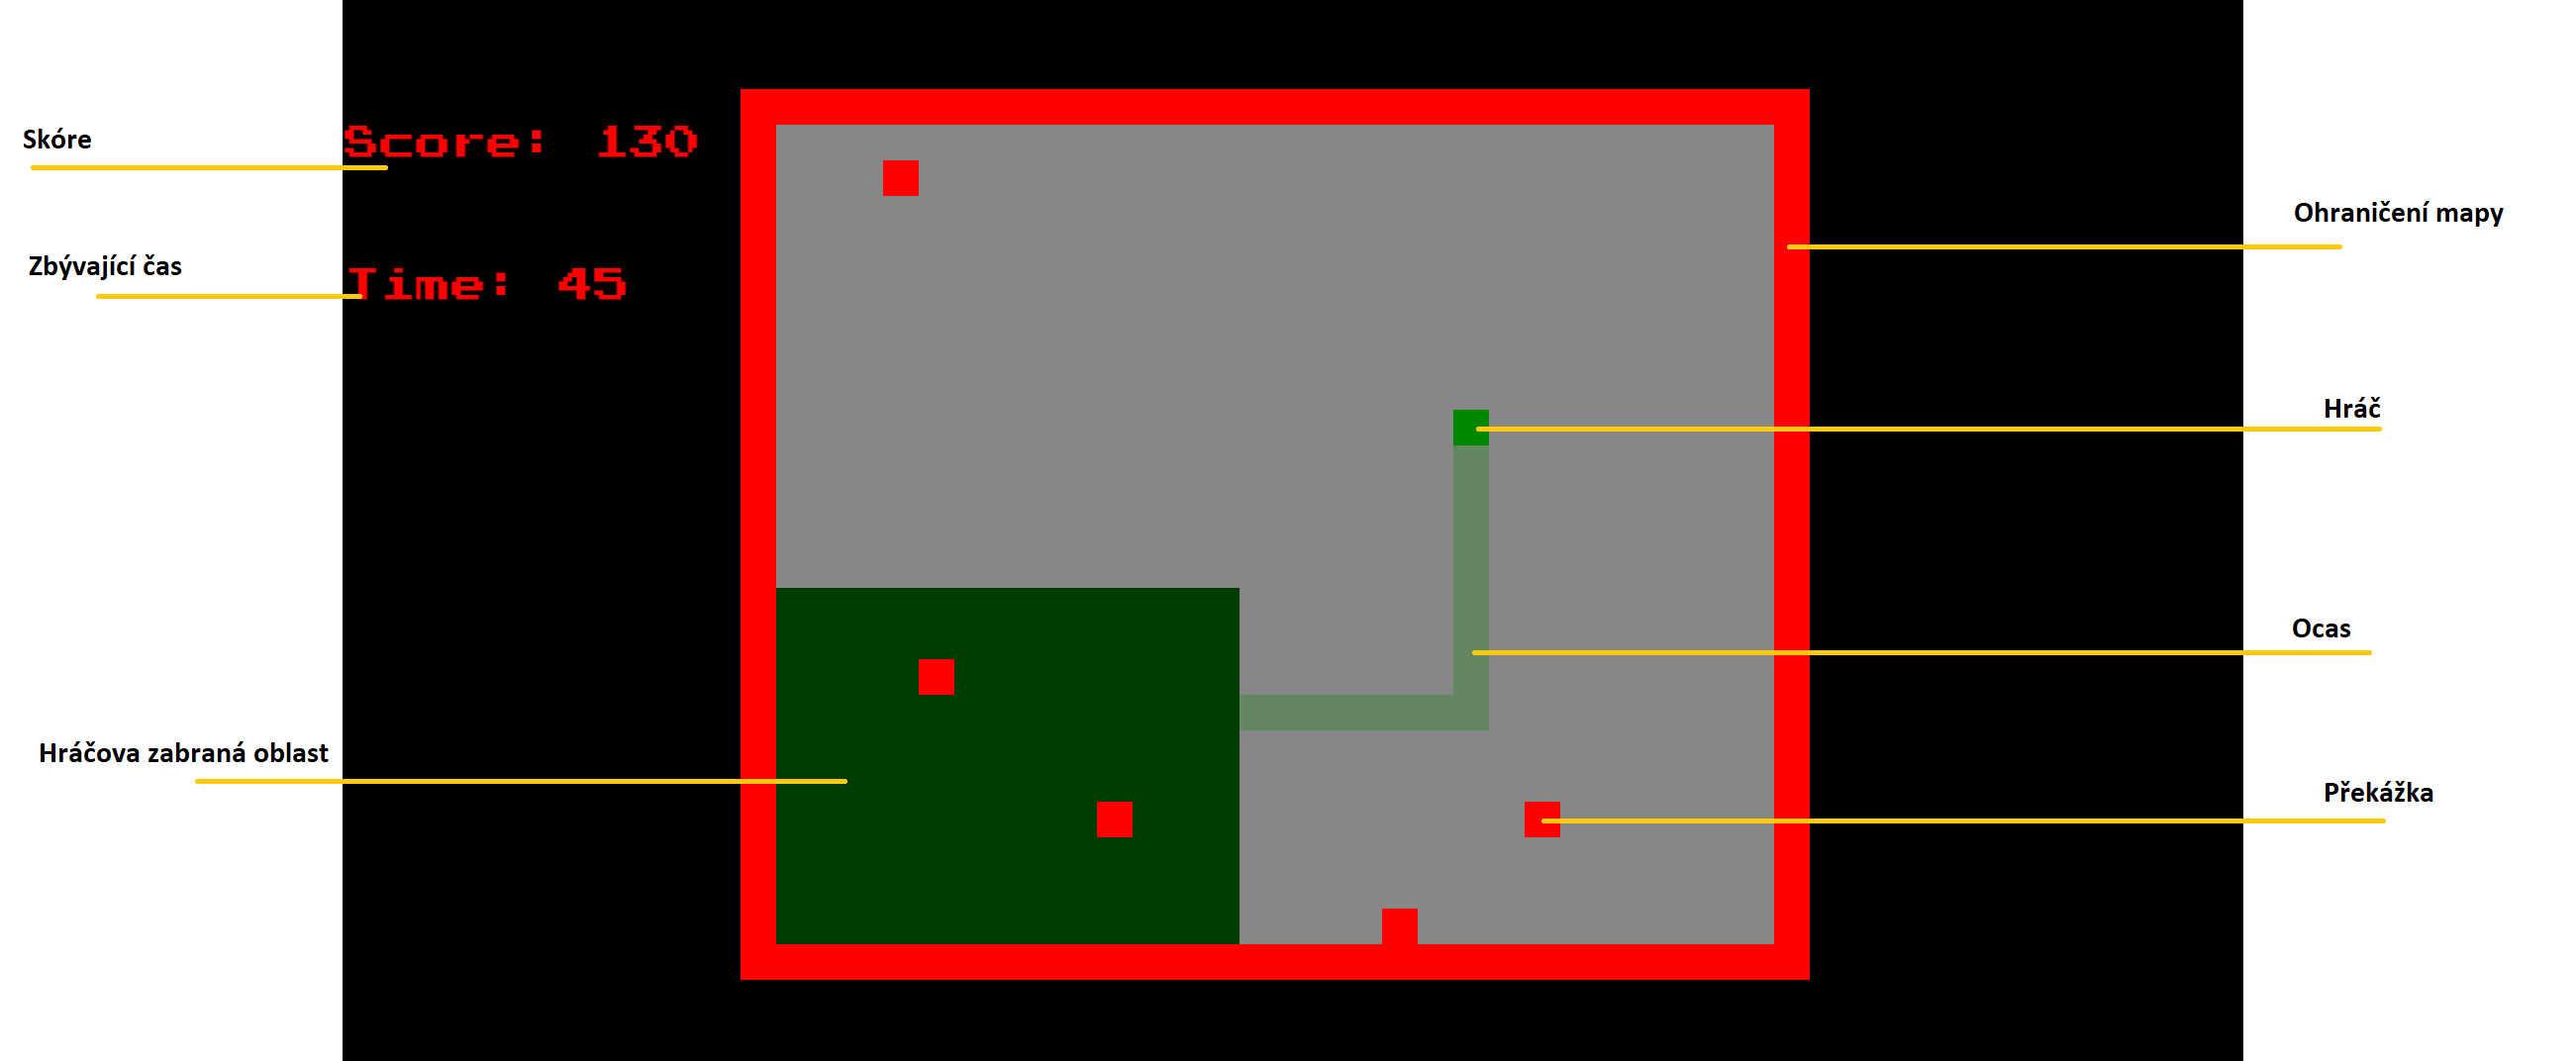
\includegraphics[width=\textwidth]{images/onePlayerGame_desc.png}
    \caption{Hra pro jednoho hráče}
\end{figure}
Pohyb hráče je pomocí kláves WASD.
\begin{itemize}
    \item W = Pohyb nahoru
    \item A = Pohyb doleva
    \item S = Pohyb dolů
    \item D = Pohyb doprava
\end{itemize}
Pokud hráč dojede zpět do své zabrané oblasti, zabere se pole mezi ocasem a hráčovou oblastí. \\
Snažíte se vyhnout překážkám a ani nenarazit do ohraničení mapy. \\
Vlevo nahoře jde vidět zbývající čas a vaše momentální skóre.
\newpage
\section{Hra pro dva hráče}
Tato obrazovka se načte po stisku tlačítka 2 Player (2 hráči).
\begin{figure}[H]
    \centering
    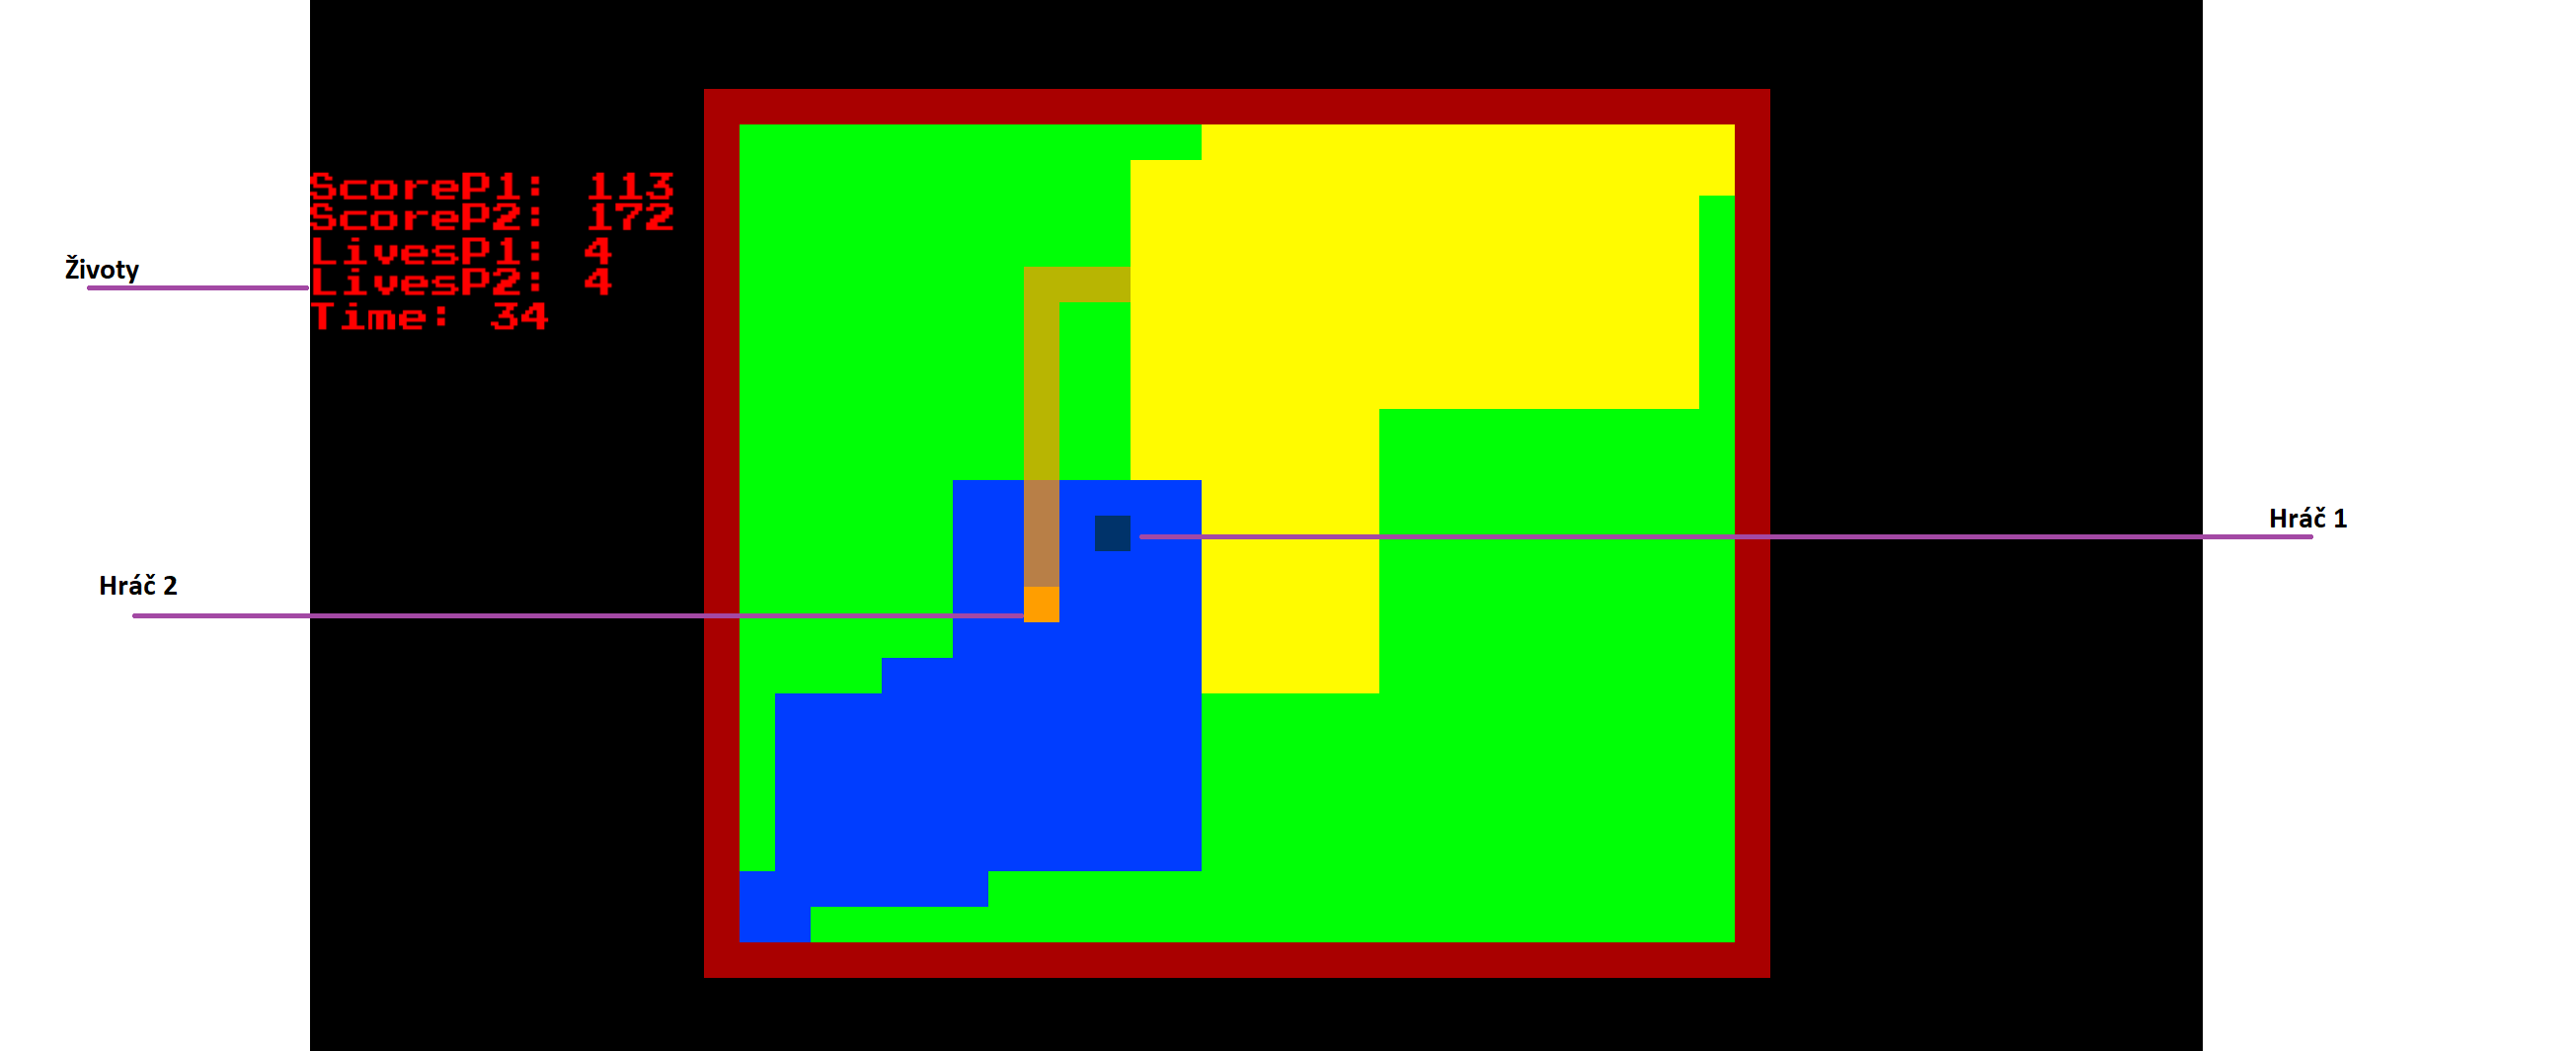
\includegraphics[width=\textwidth]{images/twoPlayerGame_desc.png}
    \caption{Hra pro dva hráče}
\end{figure}
Pokud hrajete hru pro dva hráče druhý hráč se ovládá klávesy IJKL.
\begin{itemize}
    \item I = Pohyb nahoru
    \item J = Pohyb doleva
    \item K = Pohyb dolů
    \item L = Pohyb doleva
\end{itemize}
V tomto režimu soupeříte s protihráčem. Každý hráč se snaží zabrat co nejvíce polí.
Protihráče můžete zabít, když mu přejedete přes ocas, ale jenom pokud je mimo své pole.
Hra končí pokud jednomu z hráčů dojdou životy, nebo vyprší časový limit.
Vyhraje ten hráč, který má větší skóre.
\chapter{Nastavení}
Tato obrazovka se načte po stisku tlačítka Settings (Nastavení).
\begin{figure}[H]
    \centering
    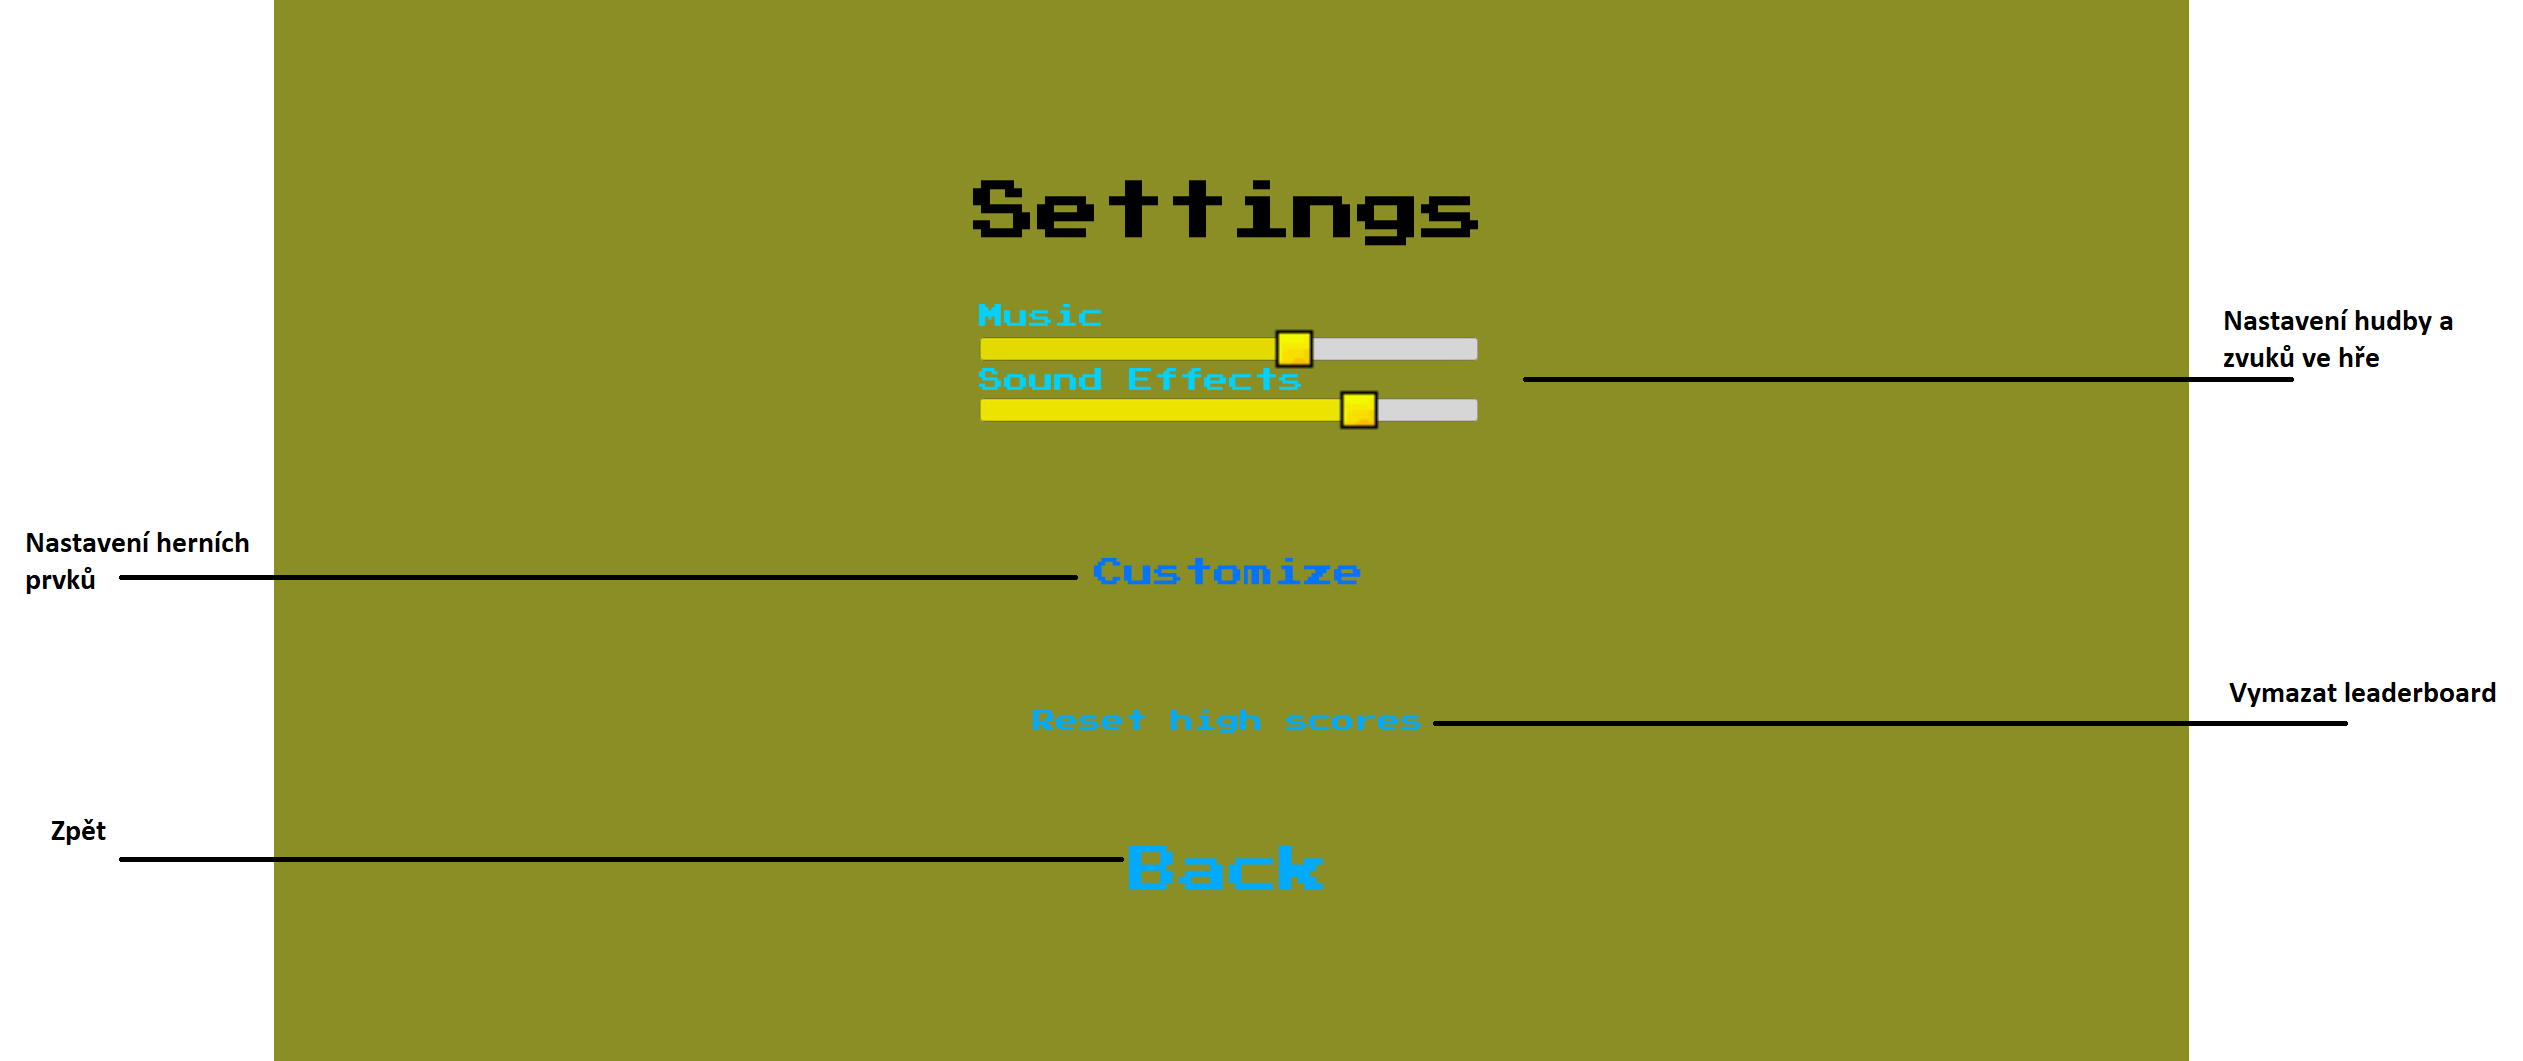
\includegraphics[width=\textwidth]{images/settings_desc.png}
    \caption{Nastavení}
\end{figure}
Na této obrazovce lze nastavit věci související s hrou.
Můžete ztišit zvuky, vynulovat žebříček nebo pomocí tlačítka customize se přesunout na novou obrazovku, kde lze nastavit různé herní prvky.
\newpage
\begin{figure}[H]
    \centering
    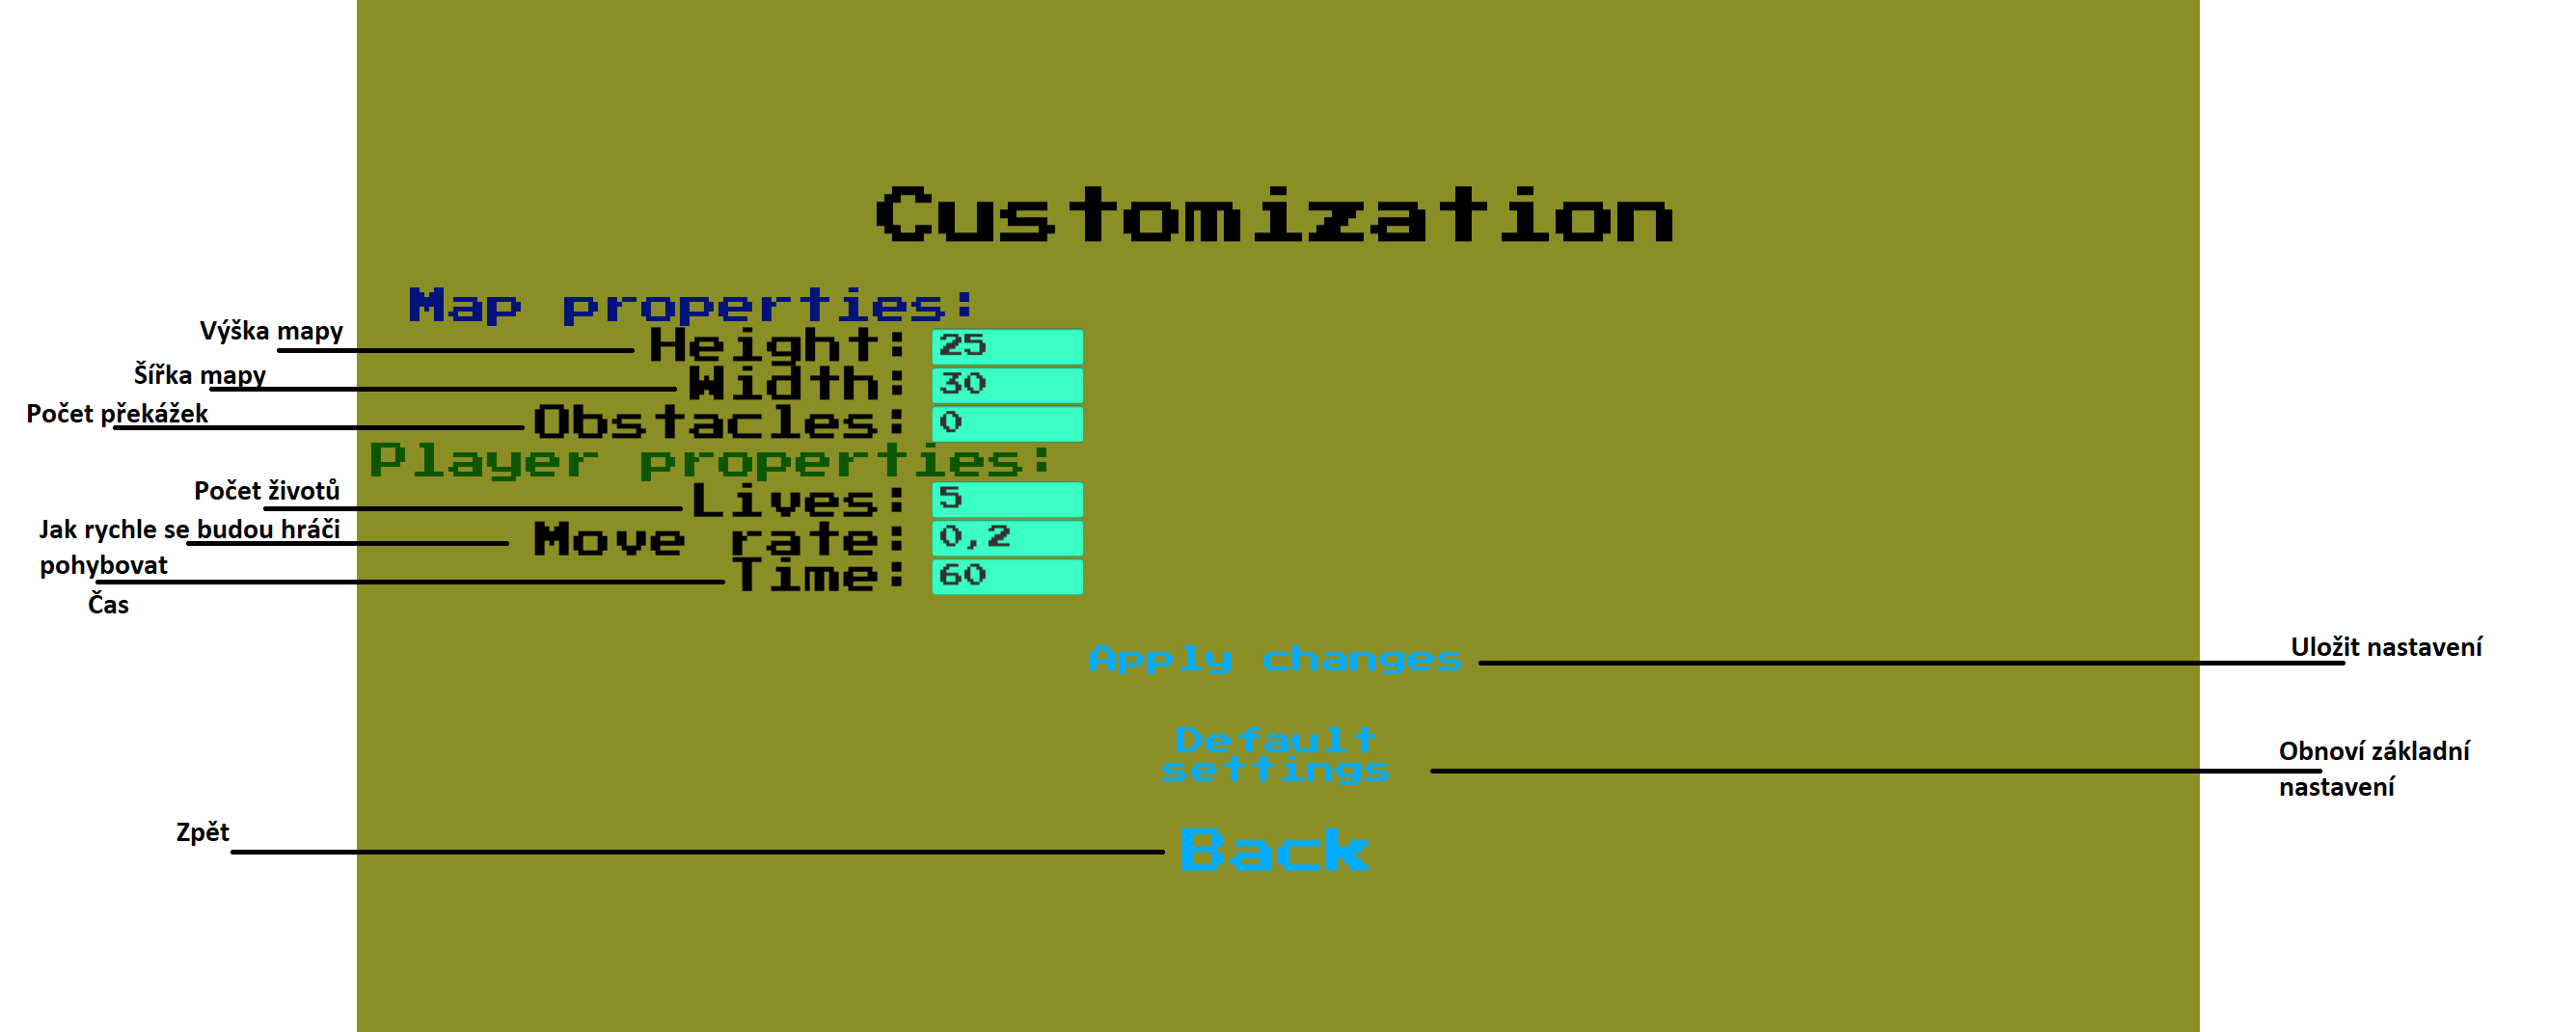
\includegraphics[width=\textwidth]{images/customization_desc.png}
    \caption{Přizpůsobení}
\end{figure}
Na této obrazovce se mění herní prvky. Lze tu změnit velikost mapy, počet překážek, životy (pro mód 2 hráčů), move rate (jak rychle se budou hráči pohybovat) a čas.
Pokud chcete změny uložit, klikněte na tlačítko apply changes.
Pokud chcete obnovit základní nastavení, můžete tak udělat pomocí tlačítka default settings.
Tlačítko back vás vrátí na předchozí obrazovku.
\end{document}
